\section{Gesti�n de clientes}
Este componente es el responsable de la gesti�n de los datos de clientes. Adem�s
de las funcionalidades b�sicas de ABM, este componente permite acciones tales
como validar clientes para realizar las operaciones que requieren de autenticaci�n.

\begin{figure}[H]
\centering
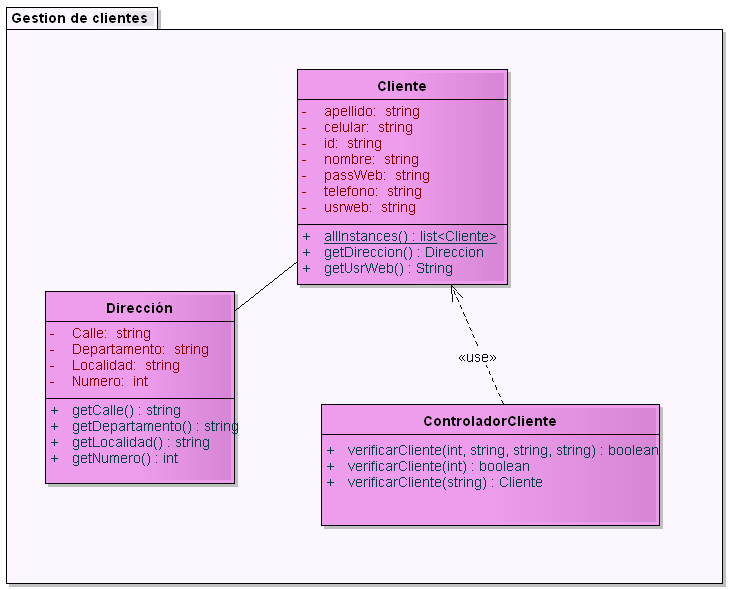
\includegraphics[height=12cm]{./figuras/compCliente.png}
\caption{Clases del componente de gesti�n de clientes}
\end{figure}

Como se describiera en \ref{metodosEstaticos}, la clase Cliente tiene m�todos 
est�ticos as� como m�todos convencionales que permiten llevar a cabo las tareas
de ABM. Sin embargo, como tambi�n es necesaria la funcionalidad adicional de validaci�n
de usuarios, en este caso se implementa un objeto Controlador que es responsable de
llevar a cabo estas tareas. Esto se hace para respetar SRP.

Las implementaciones de los m�todos de estas clases son relativamente sencillas.
El Controlador realiza b�squedas en el conjunto de instancias para chequear los
datos requeridos por la interfaz, y responde en funci�n de los mismos. En principio
no parecen ser necesarios algoritmos sofisticados de b�squeda, pero eventualmente
se podr�a modificar la implementaci�n de dichos m�todos manteniendo su interfaz
para mejorar la eficiencia si se lo juzgara necesario. La encapsulaci�n que provee
el objeto hace que estos cambios no afecten al resto del sistema puesto que tanto
la signatura como la sem�ntica de los m�todos se mantendr� intacta.

\subsection{Modelado de escenarios}
\subsubsection{Validaci�n de un cliente}
Cuando se desea ingresar un pedido remoto es necesario ingresar el cliente (esto es opcional si el pedido es local). Para hacer esto, se escriben los datos del cliente, y se realiza la validaci�n. Si es correcta se devuelve al cliente, sino se devuelve NULL.

Por ejemplo consideremos el caso en el que se quiere validar un usuario por su nombre de usuario web y que el cliente existe. Tambi�n por simplicidad modelaremos el caso en el que el segundo cliente que toma en la busqueda es el adecuado. En general hay que hacer un loop hasta encontrar un cliente, pero para no agregar ruido consideraremos ese caso

\begin{figure}[H]
\centering
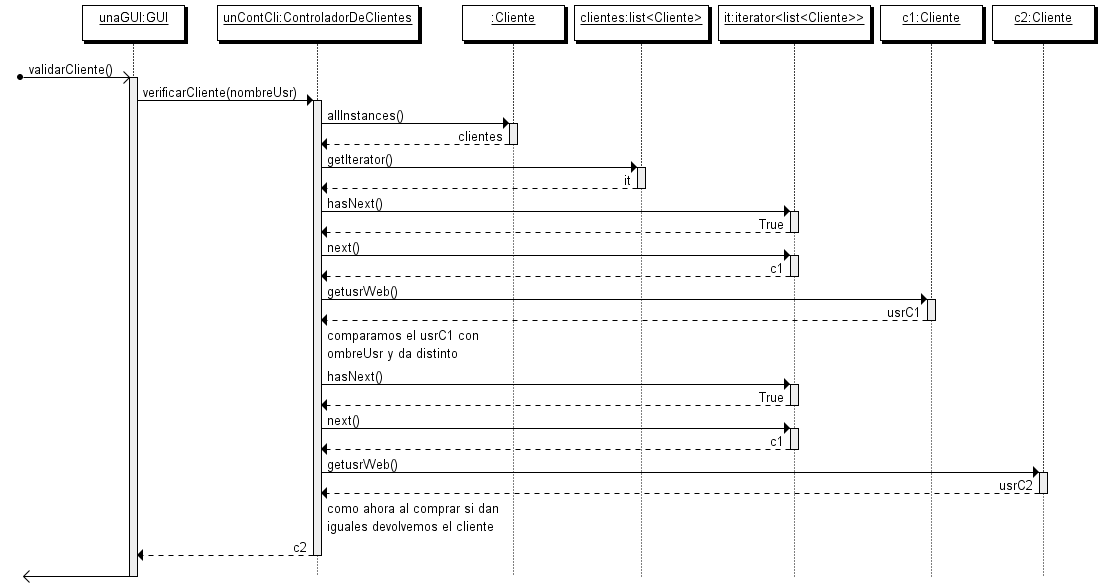
\includegraphics[height=9cm]{./figuras/validarCliente.png}
\caption{Validaci�n de un cliente}
\end{figure}
% TODO: hacer algun DS, la verdad que no hay gran cosa para poner ac�
